\chapter{Optimisation}\label{Ch-Optim}\index{optimisation}
\begin{abstract}
Ce chapitre va nous permettre de revenir sur les multiplicateurs de Lagrange dont nous avons déjà eu l'occasion de parler en plusieurs endroits de ce document, et dont l'intérêt doit être assez clair pour le lecteur à ce niveau du document.

Nous allons donc prendre un peu de temps pour mieux détailler leur utilisation, en particulier pour transformer une formulation variationnelle assortie d'un critère objectif à atteindre (le tout soumis à un certain nombre de contraintes) à l'aide de ce que l'on appelle le lagrangien, et que nous avions très brièvement évoqué au paragraphe~\ref{Sec-MultLag}).

Nous nous intéresserons aussi bien au cas où la fonction objectif est définie par des paramètres, qu'au cas de l'optimisation de forme.
\end{abstract}

\medskip
Un problème d'optimisation nécessite de fournir:
\begin{itemize}
   \item un \textcolorblue{modèle} décrivant le problème: il s'agit généralement d'une équation aux dérivées partielles;
   \item un \textcolorblue{critère} (ou des critères) que l'on cherche à minimiser ou à maximiser (c'est la fonction objectif, ou fonction coût);
   \item un \textcolorblue{ensemble admissible} de variables d'optimisation. Cet ensemble prend en compte les éventuelles \textcolorblue{contraintes} que l'on impose aux variables.
\end{itemize}

\medskip
Dans ce document, visant un public plutôt mécanicien, nous nous intéresserons essentiellement à de l'optimisation de «structures», et nous envisagerons les cas suivants:
\begin{itemize}
   \item l'optimisation \textcolorblue{paramétrique} où l'on dispose d'un nombre réduit de variables qui paramètrent la structure (par exemple l'épaisseur d'une plaque, l'orientation des plis d'un composite...). Nous verrons que des problèmes d'\textcolorblue{homogénéisation} entrent dans ce cadre;
   \item l'optimisation \textcolorblue{géométrique}: il s'agit du cas où l'on souhaite faire varier toute ou partie de la forme des frontières, mais \textcolorred{sans} changer la topologie de la pièce, i.e. sans ajouter ou supprimer de «trous»;
   \item l'optimisation \textcolorblue{topologique}: c'est le cas le plus général d'optimisation de forme d'une structure. On cherche à trouver la meilleure forme possible sans restriction, i.e. quitte à modifier la topologie.

   Si l'on s'en sort en 2D en remarquant qu'une topologie est caractérisée par le nombre de composantes connexes des bords, cela est plus compliqué en 3D où il faut en plus tenir compte du nombre d'anses ou de boucles de la structure.
\end{itemize}

Notre présentation de l'optimisation se concentrera sur l'\textcolorblue{approche continue}, l'approche discrète n'étant que très brièvement mentionnée au paragraphe~\ref{Sec-OptDisc} afin de justifier notre choix de l'optimisation continue.

\medskip
\begin{histoire}%
\ifVersionDuDocEstVincent\fontfamily{cmr}\selectfont\fi
Le mot «optimiser» a pour origine latine «optimum» qui signifie le meilleur.
Il s'agit donc de faire les choses de la meilleure façon qui soit, ou encore de concevoir la meilleure des solutions possibles en terme d'objectif prescrit (minimisation ou maximisation) et répondant à un ensemble de contraintes.
L'optimisation commence avec le calcul des variations, même si des exemples plus anciens peuvent être trouvés.

\medskip
Lié à la mythologie de la création de Carthage, résolu élégamment par la reine Didon\index[aut]{Didon, ?, Carthaginoise}, ce problème d’isopérimétrie, connu sous le nom de \textcolorblue{«Problème de Didon»}, est sans doute l'un des plus ancien problème d'optimisation dont on trouve trace.%\\ \indent

\sbox{\MaBoiteAvecPhotos}{\setlength{\tabcolsep}{0pt}\scriptsize%
\begin{tabular}{ccc}%
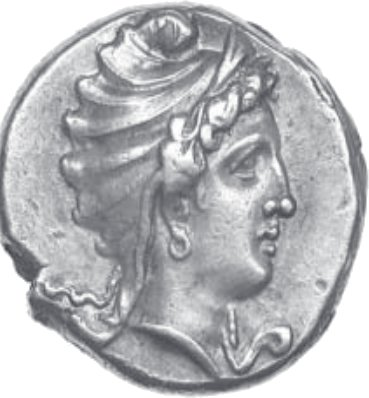
\includegraphics[height=\the\HauteurDesPhotos]{Didon}&%
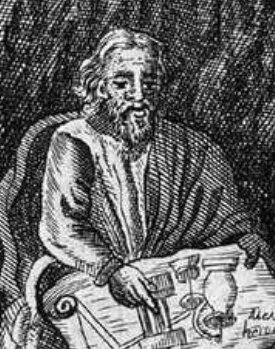
\includegraphics[height=\the\HauteurDesPhotos]{Heron}&%
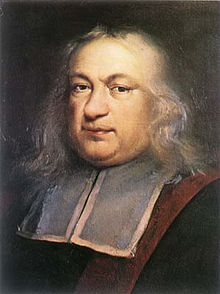
\includegraphics[height=\the\HauteurDesPhotos]{Fermat}\\%
Didon&Héron d'Alexandrie&Fermat%
\end{tabular}}
\medskip
\ImageADroite{%
%Dans \emph{Optica}, Euclide\index[aut]{Euclide, -325-- -265, Grec} se pose le problème du trajet des rayons lumineux et arrive à la conclusion qu'ils suivent un trajet optimal: les rayons incident et réfléchi sont dans le même plan, et l'angle incident et égale à l'angle réfléchi.
Dans \emph{Catoptrica}, Héron d'Alexandrie\index[aut]{Héron d'Alexandrie, 1er siècle après JC, Grec} étudie la lumière et ses réflexions. Il énonce ainsi les principes de réflexion de la lumière, principes guidés par la règle selon laquelle la nature choisit toujours le chemin le plus court.\\ \indent
Cette étude de la propagation de la lumière s'est poursuivie par l'énoncé des principes variationnels par Pierre de Fermat\index[aut]{Fermat (Pierre, de -), ?-1665, Français} et Christian Huygens\index[aut]{Huygens [ou Huyghens] (Christian), 1629-1695, Néerlandais}. Le français énonce une règle fondamentale dans la recherche d'optimum: «Lorsqu’une grandeur, par exemple l'ordonnée d'une courbe, est parvenue à son maximum ou son minimum, dans une situation infiniment voisine, son accroissement ou sa diminution est nulle.»}

\medskip
En juin 1696 dans \emph{Acta Eruditorum}, Jean Bernoulli\index[aut]{Bernoulli (Jean), 1667-1748, Suisse} reprend un problème initialement posé par Galilée.\index[aut]{Galilée (Galileo Galilei), 1564-1642, Italien}
Il s'agit du problème de la \textcolorblue{courbe brachistochrone} que l'on peut formuler comme suit: quelle est la forme de courbe joignant deux points donnés dans un plan vertical, telle qu'un point matériel, soumis uniquement à la pesanteur et initialement sans vitesse, la parcourt en un temps minimal? [Galilée pensait avoir résolu le problème et que la solution était un arc de cercle] Très rapidement, Leibniz\index[aut]{Leibniz (Gottfried Wilhelm), 1646-1716, Allemand} propose une solution à Jean Bernoulli, mais sans qu'il reconnaisse la courbe en question. C'est Jean Bernoulli, qui dispose de deux solutions, qui reconnaît un arc de cycloïde commençant avec une tangente verticale. Tous deux décident de différer la publication de leurs solutions pour laisser à d'autres la possibilité d'aborder le problème. Celui-ci fut également résolu par Jacques Bernoulli,\index[aut]{Bernoulli (Jacques), 1654-1705, Suisse} Newton,\index[aut]{Newton (Isaac, Sir -), 1643-1727, Anglais} L'Hôpital\index[aut]{Hopital@L'Hôpital (Guillaume François Antoine de -), 1661-1704, Français} et Tschirnhaus.\index[aut]{Tschirnhaus (Ehrenfried Walther von -), 1651-1708, Allemand}
Les méthodes imaginées pour sa résolution amenèrent à développer la branche des mathématiques qu'on appelle le \textcolorblue{calcul des variations}.

\sbox{\MaBoiteAvecPhotos}{\setlength{\tabcolsep}{0pt}\scriptsize%
\begin{tabular}{ccc}%
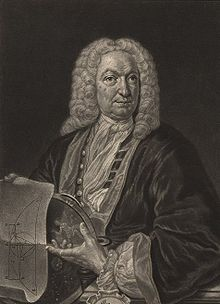
\includegraphics[height=\the\HauteurDesPhotos]{Bernoulli_Jean}&%
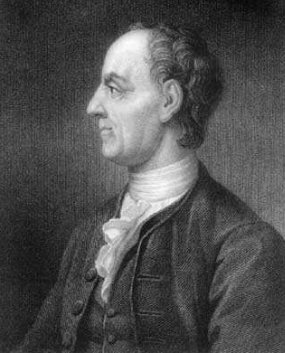
\includegraphics[height=\the\HauteurDesPhotos]{Euler6}&%
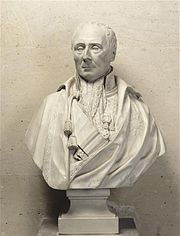
\includegraphics[height=\the\HauteurDesPhotos]{Lagrange2}\\%
J. Bernouilli&Euler&Lagrange%
\end{tabular}}
\medskip
\ImageAGauche{%
La solution de Jean Bernoulli était fondée sur une analogie avec la propagation de la lumière et le principe de Fermat, ainsi que la loi de Descartes.\index[aut]{Descartes (René), 1596-1650, Français} Celle de Leibniz, était fondée sur l'approximation de la courbe par des lignes brisées et était le premier pas vers l'équation d'Euler-Lagrange.\index[aut]{Euler (Leonhard Paul), 1707-1783, Suisse}\index[aut]{Lagrange (Joseph Louis, comte de -), 1736-1813, Italien} Le second pas a été accompli par Euler qui a ébauché, à partir de considérations géométriques, la méthode des «petites variations»; vers le milieu du dix-huitième siècle Joseph-Louis Lagrange a donné sa forme actuelle à la solution d'Euler. Legendre\index[aut]{Legendre (Adrien-Marie), 1752-1833, Français} a complété l'équation d'Euler-Lagrange, qui est une condition du premier ordre, par la condition du second ordre qui porte son nom.\\ \indent
Ces résultats ont été rassemblés par Lagrange dans sa \emph{Théorie des fonctions analytiques}, parue en 1797, et dans laquelle on lit:
«On peut les réduire à ce principe général. Lorsqu'une fonction de plusieurs variables doit être un maximum ou minimum, et qu'il y a entre ces variables une ou plusieurs équations, il suffira d'ajouter à la fonction proposée les fonctions, qui doivent être nulles, multipliées chacune par une quantité indéterminée, et de chercher ensuite le maximum ou minimum comme si les variables étaient indépendantes; les équations que l'on trouvera combinées avec les équations données, serviront à déterminer toutes les inconnues». \textcolorgris{La démarche est on ne peut plus claire, et c'est celle que nous suivrons Ces «quantités indéterminées» sont bien les multiplicateurs de Lagrange. Tout est dit!}}
Il revenait à Weierstrass,\index[aut]{Weierstrass (Karl Theodor Wilhelm), 1815-1897, Allemand} en 1879, de définir la notion d'extremum fort et d'établir la condition qui porte son nom. Les travaux de Jacobi\index[aut]{Jacobi (Carl Gustav Jakob), 1804-1851, Allemand} et Hamilton,\index[aut]{Hamilton (William Rowan, Sir -), 1805-1865, Irlandais} contemporains de ceux de Weierstrass, ont permis de donner sa forme définitive à la solution de Jacques Bernoulli déjà mentionnée. Les principaux résultats du calcul des variations classique avaient dès lors été obtenus.

\medskip
La formulation intégrale quant à elle a été peaufinée à la fin du \textsc{xix}\fup{e} siècle et au début du \textsc{xx}\fup{e} siècle.
Les économistes s'intéresseront également à ces théories.
En 1939, Leonid Kantorovich\index[aut]{Kantorovitch (Leonid Vitalievitch), 1912-1986, Russe} invente la programmation linéaire. La formulation générale des problèmes de programmation linéaire quant à elle sera finalisée en 1947 par George Dantzig\index[aut]{Dantzig (George Bernard), 1914-2005, Américain}, qui invente par ailleurs la méthode du simplexe. On parle aussi de «recherche opérationelle» pendant la seconde guerre mondiale, puis de programmation linéaire, et enfin de programmation non-linéaire.
Le calcul des variations a connu un profond renouveau dans les années 1950 avec le développement de la théorie de la \textcolorblue{commande optimale}, sous l'impulsion de Lev Pontriaguine\index[aut]{Pontriaguine (Lev Semionovitch), 1908-1988, Russe} et Richard Bellman\index[aut]{Bellman (Richard Ernest), 1920-1984, Américain}. 

Le calcul des variations reste en mathématiques un domaine fort actif, et les mathématiciens qui ont contribué à son développement sont extrêmement nombreux.
\end{histoire}

\ifVersionDuDocEstVincent\newpage\else\medskip\fi
\section{Théorie de l'optimisation}

\subsection{Existence et unicité d'un minimum}
\begin{definition}[Minima]
Soient~$V$ un espace de Banach et~$K\subset V$ un sous-ensemble non vide. Soit~$J: V\rightarrow\RR$ le critère (i.e. la fonction objectif). On considère le problème:
\begin{equation}
\inf_{v\in K} J(v)
\end{equation}

On dit que~$u$ est un \textcolorblue{minimum local} de~$J$ sur~$K$ si:
\begin{equation}
u\in K \quad\text{ et }\quad \exists\delta>0, \forall v\in K, 
\|v-u\|<\delta \Rightarrow J(v)\ge J(u)
\end{equation}

On dit que~$u$ est un \textcolorblue{minimum global} de~$J$ sur~$K$ si:
\begin{equation}
u\in K \quad\text{ et }\quad J(v)\ge J(u), \forall v\in K
\end{equation}
\end{definition}

\begin{definition}[Suite minimisante]
Une \textcolorblue{suite minimisante} du critère~$J$ sur~$K$ est une suite~$(u^n)_{n\in\NN}$ telle que:
\begin{equation}
u^n\in K, \forall n \quad\text{ et }\quad \lim_{n\rightarrow\infty} J(u^n)=\inf_{v\in K} J(v)
\end{equation}
Par définition de l'infimum de~$J$ sur~$K$, une telle suite existe toujours.
\end{definition}
Évidemment, nous allons nous intéresser à l'optimisation en dimension finie, et pour cela, nous nous servirons du résultats suivant:
\begin{theoreme}[Optimisation en dimension finie~$V=\RR^N$]
Soit~$K$ un ensemble fermé non vide de~$\RR^N$, et~$J$ une fonction continue sur~$K$ à valeurs dans~$\RR$ vérifiant la propriété \textcolorblue{infinie à l'infini} suivante:
\begin{equation}\label{Eq-infinieinfini}\colorblue
\text{Quelle que soit la suite } (u^n)_{n\in\NN} \text{ dans }K,
\quad \lim_{n\rightarrow\infty}\|u^n\|=+\infty \Rightarrow \lim_{n\rightarrow\infty}J(u^n)=+\infty
\end{equation}
alors il existe au moins un point de minimisation de~$J$ sur~$K$.

De plus, on peut extraire de toute suite minimisante de~$J$ sur~$K$ une sous-suite convergeant vers un point de minimum sur~$K$.
\end{theoreme}
\begin{remarque}
Le théorème précédent n'est pas toujours vérifié en dimension infinie: une fonction continue sur un fermé borné n'atteint pas toujours son minimum.
\end{remarque}

\medskip
Afin d'obtenir des résultats d'existence, on rajoute une hypothèse de convexité.
\begin{definition}[Convexité]
Un ensemble~$K\subset V$ est dit \textcolorblue{convexe} si:
\begin{equation}
\forall x,y\in K, \forall \theta\in \intff01, \text{ l'élément }
(\theta x+(1-\theta)y) \in K
\end{equation}

Une fonction~$J$ définie sur un ensemble convexe non vide~$K$ et à valeurs dans~$\RR$ est dite \textcolorblue{convexe} sur~$K$ si et seulement si:
\begin{equation}
J(\theta x+(1-\theta)y) \le \theta J(x)+(1-\theta)J(y), \quad \forall x,y\in K, \forall \theta\in \intff01
\end{equation}

Si de plus l'inégalité précédente est stricte lorsque~$x\ne y$ et~$\theta\in \intoo01$, alors la fonction~$J$ est dite \textcolorblue{strictement convexe}.
\end{definition}
On dispose alors du résultat suivant d'existence:
\begin{theoreme}[Existence du minimum]
Soient~$K$ un convexe fermé non vide d'un espace de Banach réflexif~$V$, et~$J$ une fonction convexe continue sur~$K$ qui est infinie à l'infini dans~$K$, i.e. qui vérifie l'équation~(\ref{Eq-infinieinfini}), alors il existe un minimum de~$J$ sur~$K$.
\end{theoreme}
\begin{remarque}[Remarques]
\textcolorgris{En toute généralité, ce théorème reste valable si~$V$ est le dual d'un espace de Banach séparable.}
\par\noindent
\textcolorgris{Le fait que~$V$ soit un espace de Banach réflexif correspond au fait que~$(V')'=V$ (avec~$V'$ le dual de~$V$).}
\par\noindent
\textcolorgreen{Enfin et surtout, ce théorème est vrai dans tous les espaces que l'on rencontre habituellement dans nos problématiques, en particulier pour les espace~$L^p(\Omega)$ pour~$1<p\le\infty$.}
\end{remarque}
\begin{theoreme}[Unicité du minimum]
Si de plus la fonction~$J$ est strictement convexe, alors il existe au plus un point de minimum.
\end{theoreme}
\begin{theoreme}
Si la fonction~$J$ est convexe sur un ensemble convexe~$K$, alors tout point de minimum local de~$J$ sur~$K$ est un minimum global.
\end{theoreme}
On voit donc tout l'intérêt de vérifier que notre fonction objectif est convexe. Un exemple d'un tel problème en mécanique est la minimisation de l'énergie.

\medskip
\subsection{Différentiabilité et optimalité}

Nous avons déjà présenté au paragraphe~\ref{Sec-Differentielle}, à l'équation~(\ref{Eq-Differentielle}), la différentielle.\index{différentielle} Si une fonction peut être approchée par une forme linéaire (la différentielle), alors on dit également qu'elle est \textcolorblue{différentiable au sens de Fréchet}.\index{dérivée!au sens de Fréchet}\index[aut]{Fréchet (Maurice René), 1878-1973, Français}

Réécrivons la définition de la différentielle dans le cas de la fonction objectif~$J$.
\begin{definition}[Différentiabilité au sens de Fréchet]
Soit~$V$ un espace de Banach. On dit que la fonction~$J$, définie au voisinage de~$u\in V$ et à valeurs dans~$\RR$, est \textcolorblue{différentiable au sens de Fréchet} en~$u$ s'il existe une forme linéaire~$L\in V'$, continue sur~$V$, telle que:
\begin{equation}
J(u+v) = J(u) + L(v) + o(v), \quad \text{ avec } \lim_{v\rightarrow0} \dfrac{|o(v)|}{\|v\|}=0
\end{equation}
On appelle~$L$ la différentielle (ou la dérivée, ou le gradient) de~$J$ en~$u$ que l'on note~$L=J'(u)$, ou encore~$L(v)=\langle J'(u),v\rangle_{V',V}$.
\end{definition}
\begin{remarque}[Remarques]
Si~$V$ est un espace de Hilbert, alors le théorème de représentation de Riesz-Fréchet\index{théorème!de représentation de Riesz-Fréchet}\index[aut]{Riesz (Frigyes), 1880-1956, Hongrois}\index[aut]{Fréchet (Maurice René), 1878-1973, Français}, donné par l'équation~(\ref{Eq-Th-RF}), permet d'identifier~$V$ à son dual~$V'$. Il existe donc un unique~$p\in V$ tel que~$\langle p,v\rangle = L(v)$. On note~$p=J'(u)$.
\par\noindent
Cette identification~$V=V'$ est utilisée si $V=\RR^N$ ou~$V=L^2(\Omega)$.
\par\noindent\colorgreen
En pratique, il est plus simple de calculer la \textcolorblue{dérivée directionnelle}\index{dérivée!directionnelle}:
\begin{equation}
j'(0) = \langle J'(u),v\rangle_{V',V}
\end{equation}
avec~$j(t)=J(u+tv)$.\colorblack
\end{remarque}

\begin{remarque}[\normalsize Lien entre minimisation et formulation variationnelle]
\normalsize Nous nous proposons de retrouver les résultats du paragraphe~\ref{Sec-MultLag}.

Soient~$a(.,.)$ une forme bilinéaire symétrique (continue coercitive) et~$f(.)$ une forme linéaire continue.
On considère la fonction~$J(u)=\frac12a(u,u)-f(u)$.
On pose, comme ci-dessus, $j(t)=J(u+tv)$. On a donc:
\[ j(t)=\frac{t^2}2a(v,v)+t\left(a(u,v)-f(v)\right)+J(u) \]
On dérive~$j$ par rapport à~$t$, ce qui donne:
\[ j'(t)=ta(v,v)+a(u,v)-f(v) \]
Par définition, on a~$j'(0)=\langle J'(u),v\rangle_{V',V}$, donc:
\[ \langle J'(u),v\rangle_{V',V} = a(u,v)-f(v) \]

La condition~$J'(u)=0$ est une formulation variationnelle.
On peut ainsi démontrer l'\textcolorblue{équivalence entre la minimisation de l'énergie~$J(u)$ et la résolution de la formulation variationnelle.}

Ce résultat est fondamental (et souvent utilisé, donc à connaître). La question que l'on est en droit de se poser est alors de savoir si une telle équivalence tient toujours dans le cas général. La réponse est oui, et nous allons maintenant présenter ces résultats.
\end{remarque}

\begin{theoreme}[Inéquation d'Euler]\index[aut]{Euler (Leonhard Paul), 1707-1783, Suisse}
Soient~$K$ un ensemble connexe et~$u$ un point de~$K$. On suppose que la fonction~$J$ est différentiable en~$u$. Si~$u$ est un point de minimum \textcolorblue{local} de~$J$ sur~$K$, alors:
\begin{equation}
\langle J(u),v-u\rangle \ge 0, \quad \forall v\in K
\end{equation}

Si~$u$ vérifie cette inéquation et si~$J$ est convexe, alors~$u$ est un minimum \textcolorblue{global} de~$J$ sur~$K$.
\end{theoreme}

Si~$u$ est \textcolorblue{intérieur} à~$K$, on obtient l'\textcolorblue{équation d'Euler}:\index[aut]{Euler (Leonhard Paul), 1707-1783, Suisse}\index{équation!d'Euler}
\begin{equation}
J'(u)=0
\end{equation}

Dans le cas général, l'inéquation d'Euler est une condition nécessaire.
Pour les fonctions convexes, elle est \textcolorblue{nécessaire et suffisante}.


\medskip
\subsection{Lagrangien}\index{lagrangien}

Dans un premier temps, nous allons nous intéresser au problème de minimisation avec contraintes d'égalité. Le cas des contraintes d'inégalités sera traiter juste à la suite.

\medskip
\begin{definition}[Lagrangien (du problème de minimisation avec contraintes d'égalité)]
Nous travaillons toujours dans notre espace~$V$.
Soit~$F(v)$ une application dérivable de~$V$ dans~$\RR^M$ \textcolorgris{(i.e. $F(v)$ est un vecteur dont les composantes sont~$F_1(v)$, ..., $F_M(v)$)}.
Nous cherchons à trouver le minimum de la fonction objectif~$J(v)$ où~$v$ satisfait aux contraintes~$F(v)=0$, i.e.:
\begin{equation}\label{Eq-LagEq}
\inf_{v\in V, F(v)=0} J(v)
\end{equation}

On appelle \textcolorblue{Lagrangien} du problème, la fonction:
\begin{equation}
\mathscr{L}(v,\mu) = J(v)+\mu.F(v) = J(v) + \dsum_{i=1}^M \mu_iF_i(v), 
\quad \forall (v,\mu)\in V\times\RR^M
\end{equation}
La variable~$\mu\in\RR^M$ est appelée \textcolorblue{multiplicateur de Lagrange}\index{multiplicateurs de Lagrange}\index[aut]{Lagrange (Joseph Louis, comte de -), 1736-1813, Italien} pour la contrainte~$F(v)=0$.
\end{definition}

Un premier résultat est que le problème de minimisation précédent est équivalent à:
\begin{equation}
\inf_{v\in V, F(v)=0} J(v) = \inf_{v\in V} \sup_{\mu\in\RR^M} \mathscr{L}(v,\mu)
\end{equation}
et l'on dispose du théorème suivant:
\begin{theoreme}[Stationnarité du Lagrangien]
On suppose que~$J$ et~$F$ sont continûment dérivables au voisinage de~$u\in V$ tel que~$F(u)=0$. Si~$u$ est un minimum local, et si les vecteurs~$(F'_i(u))_{1\le i\le M}$ sont linéairement indépendants, alors il existe des multiplicateurs de Lagrange~$\lambda_1$, ..., $\lambda_M\in\RR$ tels que:
\begin{equation}
\dfrac{\partial\mathscr{L}}{\partial v}(u,\lambda) = J'(u)+\lambda.F'(u)=0
\quad \text{ et }\quad
\dfrac{\partial\mathscr{L}}{\partial \mu}(u,\lambda) = F(u)=0
\end{equation}
\end{theoreme}

\medskip
Intéressons-nous maintenant au problème de \textcolorblue{minimisation avec contraintes d'inégalité}.
Il s'agit du même problème que précédemment, mais la relation~(\ref{Eq-LagEq}) est remplacée par la relation:
\begin{equation}\label{Eq-LagIneq}
\inf_{v\in V, F(v)\le0} J(v)
\end{equation}
où~$F(v)\le0$ signifie que pour tout~$1\le i\le M$, $F_i(v)\le0$

\begin{definition}
Soit~$u$ tel que~$F(u)\le0$.
L'ensemble~$I(u)=\{i\in\{1, ..., M\}, F_i(u)=0\}$ est appelé \textcolorblue{ensemble des contraintes actives} en~$u$.
On dit que les contraintes d'inégalité sont \textcolorblue{qualifiées} en~$u\in K$ si la famille~$(F'_i(u))_{i\in I(u)}$ est libre.
\end{definition}

\begin{definition}[Lagrangien (du problème de minimisation avec contraintes d'inégalité)]
On appelle \textcolorblue{Lagrangien} du problème, la fonction:
\begin{equation}
\mathscr{L}(v,\mu) = J(v)+\mu.F(v) = J(v) + \dsum_{i=1}^M \mu_iF_i(v), 
\quad \forall (v,\mu)\in V\times(\RR^+)^M
\end{equation}
La variable \textcolorred{positive}~$\mu\in(\RR^+)^M$ est appelée \textcolorblue{multiplicateur de Lagrange}\index{multiplicateurs de Lagrange}\index[aut]{Lagrange (Joseph Louis, comte de -), 1736-1813, Italien} pour la contrainte~$F(v)\le0$.
\end{definition}

\colorgreen
\noindent\textbf{Synthèse méthodologique:} Le lagrangien (pour le problème de minimisation avec contraintes d'égalité, comme d'inégalité) est la somme de la fonction objectif et de la formulation variationnelle de l'équation d'état du problème considérée comme une contrainte \textcolorgris{(i.e. nous avons suivi à la lettre la méthode décrite par Lagrange lui-même)}.
\colorblack

\medskip
Un premier résultat est que le problème de minimisation précédent est équivalent à:
\begin{equation}
\inf_{v\in V, F(v)\le0} J(v) = \inf_{v\in V} \sup_{\mu\in(\RR^+)^M} \mathscr{L}(v,\mu)
\end{equation}
et l'on dispose du théorème suivant:
\begin{theoreme}[Stationnarité du Lagrangien]
On suppose que les contraintes sont qualifiées en~$u$ tel que~$F(u)\le0$. Si~$u$ est un minimum local, alors il existe des multiplicateurs de Lagrange~$\lambda_1$, ..., $\lambda_M\in\RR^+$ tels que:
\begin{equation}
\dfrac{\partial\mathscr{L}}{\partial v}(u,\lambda) = J'(u)+\lambda.F'(u)
= J'(u)+\dsum_{i=1}^M\lambda_iF_i'(u) =0, \quad \lambda_i\ge0, 
\quad \forall i\in\{1, ..., M\}
\end{equation}
Notons que~$\lambda_i=0$ si~$F_i(u)<0$.

En plus de la stationnarité du Lagrangien, notons que la condition~$\lambda\ge0$, $F(u)\le 0$, $\lambda.F(u)=0$ est équivalente à l'inéquation d'Euler pour la \textcolorblue{maximisation} par rapport à~$\mu$ dans le convexe fermé qu'est~$(\RR^+)^M$:
\begin{equation}
\dfrac{\partial\mathscr{L}}{\partial \mu}(u,\lambda).(\mu-\lambda)=F(u).(\mu-\lambda)\le0, \quad \forall\mu\in(\RR^+)^M
\end{equation}
\end{theoreme}

D'un point de vue pratique, $\lambda$ donne la dérivée (sans la calculer) du minimum par rapport à la contrainte.
\begin{demonstration}[Illustration]
Considérons le cas de la minimisation de~$J(u)$ sous la contrainte~$F(u)=c$.
Le Lagrangien est:
\[ \mathscr{L}(v,\mu,c)=J(v)+\mu.(F(v)-c) \]
et on se propose d'étudier la sensibilité du Lagrangien par rapport à~$c$.

Notons~$u(c)$ et~$\lambda(c)$ le point de minimum et le multiplicateur de Lagrange correspondant. On supposera évidemment qu'ils sont dérivables par rapport à~$c$. Il vient alors:
\[ \nabla_c\left(J(u(c))\right)=-\lambda(c) \]
et ainsi~$\lambda$ donne bien la dérivée (sans la calculer) du minimum par rapport à~$c$.
\end{demonstration}


\medskip
\subsection{Dualité et point selle}

Dans ce paragraphe, on va regarder comment supprimer les contraintes portant sur le problème. Pour cela, on va adjoindre au problème dit primal, un problème dual. Ce dernier est souvent plus simple que le problème primal, notamment parce qu'il ne comporte pas de contraintes. Évidemment, connaissant la solution du problème dual, on devra être en mesure de remonter à celle du problème primal.

\begin{definition}
Soit un Lagrangien~$\mathscr{L}(v,q)$.
On dit que~$(u,p)\in U\times P$ est un \textcolorblue{point selle} de~$\mathscr{L}$ sur~$U\times P$ si:
\begin{equation}
\forall q\in P, \quad \mathscr{L}(u,q) \le \mathscr{L}(u,p) \le \mathscr{L}(v,p), \forall v\in U
\end{equation}

Pour $v\in U$ et~$q\in P$, posons~$\mathcal{J}(v)=\sup_{q\in P}\mathscr{L}(v,q)$ et~$\mathcal{G}(q)=\inf_{v\in U}\mathscr{L}(v,q)$.
On appelle \textcolorblue{problème primal}:
\begin{equation}
\inf_{v\in U} \mathcal{J}(v)
\end{equation}
et \textcolorblue{problème dual}:
\begin{equation}
\sup_{q\in P} \mathcal{G}(q)
\end{equation}
\end{definition}

Pour faire le lien avec ce qui précède, plaçons nous dans le cas où~$U=V$, $P=\RR^M$, et~$\mathscr{L}(v,q)=J(v)+q.F(v)$.
Il vient alors: $\mathcal{J}(v)=J(v)$ si~$F(v)=0$ et~$\mathcal{J}(v)=+\infty$ sinon.
Par contre, il n'y a pas de contrainte pour le problème dual, si ce n'est~$q\in P=\RR^M$.

\textcolorgreen{Comme annoncé, le problème dual est plus simple que le problème primal, car il n'a pas de contrainte.}

\begin{theoreme}[Dualité forte]
Le couple~$(u,p)$ est un point selle de~$\mathscr{L}$ sur~$U\times P$ si et seulement si:
\begin{equation}
\mathcal{J}(u)=\min_{v\in U}\mathcal{J}(v) = \max_{q\in P}\mathcal{G}(q)=\mathcal{G}(p)
\end{equation}
\end{theoreme}

\textcolorgreen{Ainsi, si l'on sait résoudre le problème dual, alors on obtient la solution du problème primal grâce à une minimisation \textcolorred{sans} contrainte.}

\subsection{Maximisation}

Jusqu'à présent, nous n'avons parlé que de problème de minimisation.
Si l'on a à traiter un problème de maximisation, il suffit alors de le transformer en problème de minimisation:
\begin{equation}
\sup_{v\in V} J(v)=-\inf_{v\in V} (-J(v))
\end{equation}

\medskip
\subsection{Ensemble admissible}

Nous avons été assez vagues sur le domaine dans lequel peuvent varier les variables d'optimisation. Nous avons parlé d'espace, d'ensemble connexe...

D'un point de vue pratique, les variables (ou paramètres) ne peuvent varier qu'à l'intérieur d'un domaine admissible. Cet \textcolorblue{ensemble admissible} sera noté~$\mathscr{U}_{\text{ad}}$.

\medskip
Cet ensemble peut aussi bien comprendre:
\begin{itemize}
   \item des domaines \textcolorblue{discrets}: par exemple, 1) le nombre de plis dans un stratifié doit être un entier compris entre~$1$ et~$n$, où~$n$ est le nombre de plis maximum au-delà duquel on estime que le processus de fabrication ne sera plus performant (techniquement et/ou économiquement), 2) l'épaisseur d'une tôle peut n'avoir qu'un nombre fini de valeurs discrètes correspondant à ce qui existe en stock ou dans le commerce;
   \item que des domaines \textcolorblue{continus}: par exemple, 1) l'angle d'orientation des plis dans un stratifié est une variable continue sur~$\intff{-\pi}{\pi}$, 2) l'épaisseur d'une structure peut être vue comme une variable continue allant d'une valeur min à une valeur max données.
\end{itemize}

Lorsque nous parlerons d'optimisation géométrique (ou optimisation de forme), alors nous aurons à manipuler des contraintes du type: telle partie de la frontière peut bouger, mais sa longueur doit être constante, ou le volume total délimité doit respecter telle ou telle condition.

Nous pourrons également avoir des critères lié à l'état des contraintes ou des déformations de la structure, des critères de moindre carrés (pour atteindre par exemple un déplacement cible), une rigidité, un déplacement maximal...

\medskip
Pour prendre en compte des variables ayant des \textcolorblue{valeurs discrètes}, on peut se servir de fonctions caractéristiques.
Par  exemple: si une variable~$v$ ne peut prendre que la valeur~$\alpha$ dans un sous-domaine~$\omega\subset\Omega$ et la valeur~$\beta$ ailleurs, alors on pourra écrire:
\begin{equation}
v = \alpha \chi(x) + \beta(1-\chi(x))
\end{equation}
où~$x$ est la position du point considéré et~$\chi(x)$ la fonction caractéristique qui vaut~$1$ si~$x\in\omega$ et~$0$ sinon.

\medskip
On peut également faire varier le critère en fonction de la zone de la structure considérée.
Pour cela, notre domaine~$\Omega$ peut être décomposé en une \textcolorblue{partition}~$(\omega_i)_{1\le i\le n}$, et l'on est amené à considérer l'ensemble admissible:
\begin{equation}
\mathscr{U}^n_{\text{ad}}=\{ x\in \mathscr{U}_{\text{ad}}, x \text{ vérifie la condition } i \text{ dans } \omega_i, 1\le i\le n\}
\end{equation}

\medskip
On peut également avoir des \textcolorblue{contraintes de régularité}. C'est par exemple ce que l'on peut imposer à une épaisseur variable: non seulement celle-ci doit être comprises entre une valeur mini et une valeur maxi, mais on peut également vouloir que sa variation soit bornée, i.e. qu'elle ne varie pas trop vite, ce qui correspond à une contrainte pratique du processus de fabrication.
Ainsi, on se fixe une constante positive~$R$, et l'on travaille sur l'ensemble admissible:
\begin{equation}
\mathscr{U}^{\text{reg}}_{\text{ad}}=\{ x\in \mathscr{U}_{\text{ad}} \cap W^{1,\infty}(\Omega), \|x\|_{W^{1,\infty}(\Omega)}\le R\}
\end{equation}
Le problème reste de choisir la valeur de~$R$. En général, il n'y a d'ailleurs pas convergence quand~$R$ tend vers l'infini.
Numériquement, on préfère la contrainte de régularité:
\begin{equation}
\|x\|_{H^1(\Omega)}\le R
\end{equation}

\medskip
\subsection{L'optimisation discrète}\label{Sec-OptDisc}

On peut également discrétiser des contraintes d'optimisation. L'ensemble admissible devient alors:
\begin{equation}
\begin{split} 
\mathscr{U}^{\text{disc}}_{\text{ad}} = &\Bigg\{ \text{contraintes sur } x \text{ idem celles sur } \mathscr{U}_{\text{ad}}; ...\\  
& \left. \quad ... \text{ contraintes sur } \int x...=... \text{ remplacées par } \dsum_{i=1}^n c_ix_i = ... \right\}
\end{split}
\end{equation}
où~$\sum_{i=1}^n c_ix_i$ est une approximation de~$\int x...$.

Le problème est de calculer le gradient de~$J^{\text{disc}}$. Si l'on procède de manière directe, cela est impraticable numériquement. On passe alors par l'état adjoint (voir exemples plus bas).

\medskip
\textcolorgreen{Il n'y a pas de simplification à utiliser une approche discrète plutôt que continue:}
\begin{itemize}
   \item certes «discrétiser d'abord puis optimiser» garantit une parfait compatibilité, mais cela nécessite une parfaite connaissance du solveur numérique;
   \item alors qu'«optimiser en continu puis discrétiser», tel que présenté dans ce chapitre, est beaucoup plus simple et ne nuit pas en précision numérique si l'on choisit bien les espaces d'éléments finis.
\end{itemize}


\medskip
\subsection{Remarques sur la mise en œuvre}

Des méthodes dites «stochastiques» telles que Monte-Carlo, recuit simulé ou des algorithmes génétiques sont envisageables. Elles sont coûteuses en CPU et nous ne les aborderons pas.

Nous allons dire deux mots sur les méthodes déterministes, telles que les \textcolorblue{méthodes de gradient} (gradient optimal, gradient à pas fixe, gradient projeté) ou de Newton. Notons qu'elles fournissent un minimum local, et que, pour fonctionner, il faut disposer du gradient. \textcolorred{Ainsi, nous devrons pouvoir calculer~$J'$}. C'est d'ailleurs sur le calcul de~$J'$ que nous insisterons dans les exemples traités.

\medskip
La méthode la plus simple (et la plus sûre) pour calculer le gradient est:
\begin{equation}
\lim_{\varepsilon\rightarrow0} \dfrac{J(x+\varepsilon y)-J(x)}{\varepsilon}
=\langle J'(x),y\rangle %=\dint_\Omega J'(x)y
\end{equation}
Par linéarité on écrit: $u(x+\varepsilon y)=u(x)+\varepsilon \tilde{u}(y)$, les relations satisfaites par~$\tilde{u}(y)$ dépendant du problème considéré.
Toutefois, remarquons qu'avec cette manière de procéder~$J'(x)$ n'est pas explicite.

\medskip
Pour calculer explicitement l'expression du gradient, on utilise l'\textcolorblue{état adjoint}~$p$, qui nécessite de résoudre deux problèmes aux limites ($u$ et $p$).
Cette méthode est très efficace en pratique, c'est la meilleure possible.

D'une manière générale, on peut dire que l'état adjoint est obtenu comme stationnarité d'un lagrangien dont $p$ est le multiplicateur de Lagrange et l'équation d'état la contrainte.
De même, $J'$ est obtenu comme stationnarité de ce même Lagrangien par rapport à la variable de contrôle optimal.

Si l'équation d'état est non-autoadjointe (i.e. si la forme bilinéaire du problème n'est pas symétrique), alors l'opérateur principal de l'équation adjointe est le transposé ou l'adjoint de celui de l'équation d'état.
Par contre, même si l'équation d'état est non linéaire, l'équation adjointe est linéaire (c'est assez normal, puisque finalement, on ne s'intéresse qu'aux fluctuations en somme).

Nous n'en dirons pas plus ici, quelques exemples plus bas permettrons de voir le calcul effectif de l'état adjoint et de~$J'$.


\medskip
\section{Optimisation de forme}

Maintenant que nous avons présenté la théorie de l'\textcolorblue{optimisation continue}, nous nous proposons de dire quelques mots sur sa mise en œuvre dans le cadre de l'optimisation de forme. D'un point de vue vraiment pratique, c'est au paragraphe suivant que se trouveront les exemples, traités dans le cas d'une plaque.

\medskip
Le problème principal qui se pose est de savoir comment poser le problème, i.e. comment représenter des formes, et par suite comment définir le calcul des variations sur les formes.

\medskip
\subsection{Optimisation paramétrique}

On est dans le cas le plus simple. La géométrie ne peut pas «vraiment» varier: elle est paramétrée par des variables. L'ensemble~$\mathscr{U}_{\text{ad}}$ est donc celui défini par l'ensemble de ces variables munies de leur domaine de variation (valeur mini et maxi).

En somme, ce cas a déjà été traité auparavant, et il n'y a pas de différence dans le traitement d'un paramètre, que celui-ci représente un élément de la géométrie ou un autre type de variable.

\medskip
\subsection{Optimisation géométrique}

On rappelle que dans ce cas, la géométrie peut varier mais pas la topologie. On n'est donc pas autorisé à ajouter ou supprimer des trous.

\medskip
\subsubsection{Approche «libre»}

Généralement, le contour~$\Gamma=\partial\Omega$ est partitionné comme suit:
\begin{equation}
\Gamma = \Gamma_D \cup \Gamma_N \cup \Gamma_R
\end{equation}
où~$\Gamma_D$ est la partie où les déplacements sont imposés, considérée comme immuable; $\Gamma_N$ est la partie où les efforts extérieurs sont prescrits, également considérée comme fixe; et~$\Gamma_R$ est le reste du contour, seule partie qui peut varier (tout ou partie, auquel cas on partitionne encore en une partie fixe et une partie mobile).
On commence donc par imposer que~$\Gamma_D$ et~$\Gamma_N$ sont fixes:
\begin{equation}
\mathscr{U}_{\text{ad}}=\{ \Gamma_D \cup \Gamma_N \subset \Gamma\}
\end{equation}

Ne rien imposer de plus ne permet pas de résoudre le problème. Il nous faut des critères d'optimisation.
On veut trouver la forme optimale qui permet, par exemple, de maximiser la rigidité, ou d'obtenir un déplacement cible.
Mais cela ne suffit pas encore. Si toutes les formes sont admissibles, alors on va arriver à des solutions où l'on a des volumes nuls ou infinis, car cela répondra au mieux...
Il est donc nécessaire de contraindre la forme: 
tout d'abord, on va restreindre la géométrie à ne varier que dans un domaine~$D_0$ borné défini, ce qui se traduit par l'ajout de la condition:
\begin{equation}
\mathscr{U}_{\text{ad}}=\{ \Omega\subset D_0 \}
\end{equation}
Ensuite, par exemple, on peut décider de travailler à volume fixé~$V_0$, ce qui se traduit par:
\begin{equation}
\mathscr{U}_{\text{ad}}=\{ |\Omega|=V_0\}
\end{equation}

Nous en sommes donc à un ensemble admissible qui se présente sous la forme:
\begin{equation}
\mathscr{U}_{\text{ad}}=\{ \Omega\subset D_0 /\quad 
\Gamma_D \cup \Gamma_N \subset \Gamma \text{ et } |\Omega|=V_0 \}
\end{equation}

Mais cela n'est pas encore suffisant pour obtenir une solution.
Il est nécessaire d'ajouter que~$\Omega$ vérifie la \textcolorblue{propriété du cône uniforme}. Cette condition impose à la fois une condition sur le rayon de courbure du bord (c'est une condition pour le bord varie de manière assez lisse) et empêche la formation de petits trous.

\begin{theoreme}[D. Chenais]
Si l'ensemble admissible est:
\begin{equation}
\mathscr{U}_{\text{ad}}=\left\{ \Omega\subset D_0 \text{ tq: }
\begin{array}{l}
(i)\quad \Omega \text{ vérifie la propriété du cône uniforme}\\
(ii)\quad \Gamma_D \cup \Gamma_N \subset \Gamma \text{ et } |\Omega|=V_0 
\end{array}
\right\}
\end{equation}
alors le problème d'optimisation:
\[ \inf_{\Omega\in\mathscr{U}_{\text{ad}}} J(\Omega) \]
admet au moins une solution optimale.
\end{theoreme}

\medskip
\subsubsection{Approche «régulière»}

Une autre voie est possible pour réaliser une optimisation géométrique: c'est celle où l'on déforme progressivement le domaine initial pour arriver jusqu'au domaine final. Nous avons déjà mentionné cette manière de faire à propos des maillages au chapitre~\ref{Ch-mesh}. Nous allons pour cela utiliser la notion de \textcolorblue{transformation par difféomorphisme} du domaine initial~$\Omega_0$ de~$\RR^N$.
\textcolorgreen{Une telle approche a pour avantage d'assurer qu'au cours de la transformation le domaine reste bien topologiquement identique au domaine initial. Elle a également le gros avantage de permettre de calculer un gradient.}

\medskip
\begin{definition}[Espace des difféomorphismes]
L'espace des difféomorphismes~$\mathscr{T}$ (ou espace des bijections régulières) sur~$\RR^N$ est défini par:
\begin{equation}
\mathscr{T}=\left\{ T \text{ tel que } (T-Id) \text{ et } (T+Id)\in W^{1,\infty}(\RR^N;\RR^N)\right\}
\end{equation}
L'espace de Sobolev~$W^{1,\infty}(\RR^N;\RR^N)$ est également appelé espace des vecteurs Lipschitziens. Il est muni de:
\begin{equation}
\|\varphi\|_{W^{1,\infty}(\RR^N;\RR^N)}=\sup_{x\in\RR^N} \left(|\varphi(x)|_{\RR^N}
+|\nabla\varphi(x)|_{\RR^{N\times N}}\right) <\infty
\end{equation}
Ainsi, $\varphi$ est continue mais ses dérivées sont seulement bornées.
\end{definition}

L'\textcolorblue{espace des formes admissibles} est alors:
\begin{equation}
\mathcal{C}(\Omega_0)=\left\{ \Omega \text{ tel que: } \exists T\in\mathscr{T}, \Omega=T(\Omega_0) \right\}
\end{equation}
Attention, chaque domaine~$\Omega$ est bien paramétré par un difféomorphisme~$T$, mais celui-ci n'est pas unique.

On définit la pseudo-distance:
\begin{equation}
d(\Omega_1,\Omega_2) = \inf_{T\in\mathscr{T}/ T(\Omega_1)=\Omega_2}
\left( \|T-Id\|+\|T^{-1}-Id\|\right)_{W^{1,\infty}(\RR^N;\RR^N)}
\end{equation}

Si~$\Omega_0$ est borné, alors on peut utiliser~$C^1(\RR^N;\RR^N)$ au lieu de~$W^{1,\infty}(\RR^N;\RR^N)$.

\medskip
L'ensemble admissible est finalement:
\begin{equation}
\mathscr{U}_{\text{ad}} = \{ \Omega\in\mathcal{C}(\Omega_0) / \quad
\Gamma_D \cup \Gamma_N \subset \Gamma \text{ et } |\Omega|=V_0 \}
\end{equation}
Comme précédemment, on fixe une constante positive~$R$ (contrainte de faisabilité), et on introduit le sous-espace régulier:
\begin{equation}
\mathscr{U}_{\text{ad}}^{\text{reg}} = \{ \Omega\in\mathscr{U}_{\text{ad}}) / \quad
d(\Omega,\Omega_0)\le R \}
\end{equation}
On dispose alors du résultat suivant:
\begin{theoreme}
Si l'ensemble admissible est~$\mathscr{U}_{\text{ad}}^{\text{reg}}$ défini juste avant, alors le problème d'optimisation:
\[ \inf_{\Omega\in\mathscr{U}_{\text{ad}}^{\text{reg}}} J(\Omega) \]
admet au moins une solution optimale.
\end{theoreme}

Notons que les bords dans~$\mathscr{U}_{\text{ad}}^{\text{reg}}$ ne peuvent pas trop osciller.

\medskip
Comme~$J(\Omega)$ est paramétré par le difféomorphisme~$T$, il est possible de calculer sa dérivée.

En se limitant aux difféomorphismes de la forme~$T=Id+\theta$, avec~$\theta\in W^{1,\infty}(\RR^N;\RR^N)$, on peut dériver $\theta \rightarrow J((Id+\theta)\Omega_0)$ en~$0$, qui est strictement contractante. Ainsi, $T=Id+\theta$ est une bijection de~$\RR^N$. Il suffit d'appliquer la définition de la dérivée au sens de Fréchet. La forme linéaire est cette fois-ci appelée \textcolorblue{dérivée de forme}.

De la même manière, il est possible de définir la dérivée d'une fonction dépendant du domaine, que ce soit la dérivée eulérienne ou la dérivée lagrangienne.
Dans la mesure où la dérivée eulérienne est délicate à manipuler, on préfèrera utiliser la dérivée lagrangienne, quitte à exprimer les résultats de la dérivation eulérienne à partir de la dérivation lagrangienne.
Enfin, on peut également dériver une équation par rapport au domaine, ou une formulation variationnelle... mais nous en resterons là pour l'instant.

De toutes façons, ce n'est pas cette méthode (calculatoire) qui est utilisée en pratique, mais la \textcolorblue{méthode du Lagrangien}... dont nous avons déjà parlé auparavant.
En effet, la dérivée du Lagrangien par rapport au domaine, dans la direction~$\theta$, évaluée sur le domaine~$\Omega_0$, est égale à la dérivée directionnelle~$J'(\Omega_0)(\theta)$.
Ainsi, grâce à ce calcul, on peut obtenir de bons résultats pour~$J'(\Omega_0)$ sans passer par les dérivées de forme ou matérielle. Ce calcul nécessite toutefois que l'on connaisse la dérivabilité de~$u$ par rapport au domaine.

\medskip
Un problème implicite non évoqué est que \textcolorred{pour changer de forme, il faut pouvoir remailler ou déformer le maillage à chaque itération}.
Comme un remaillage est beaucoup plus coûteux qu'une déformation de maillage, on procède par déformation de maillage (avec toutes les précautions nécessaires sur le respect des formes d'éléments, sur le croisement des bords...) avec de temps en temps un remaillage (on ne peut pas y couper...). C'est pourquoi la mise en œuvre informatique de l'optimisation géométrique reste compliquée (surtout en 3D).

Une «Boite à outils \freefem pour l'optimisation de formes (géométrique et topologique)» est disponible sur le site de Grégoire Allaire\index[aut]{Allaire (Grégoire), ?-, Français} du CMAP~\cite{bib-AllaireOptimFF}.


\medskip
\subsection{Optimisation topologique par homogénéisation}

La restriction majeur de l'optimisation géométrique dont nous venons de parler est que l'on ne modifie pas la topologie de la structure, ce qui limite considérablement les formes possibles.
Nous allons voir maintenant comment s'affranchir de cette limitation, en présentant une méthode d'homogénéisation. Nous ne présenterons pas d'approche évolutionnaire.

\medskip
La \textcolorblue{méthode d'homogénéisation} est une méthode qui permet de rendre les problèmes bien posés en élargissant l'espace des formes admissibles.
Ces \textcolorblue{formes généralisées} seront les limites de suites minimisantes de formes classiques (ce qui augmente les possibilités, mais sans trop d'excentricité).
Ainsi, la méthode d'homogénéisation autorise comme formes admissibles des matériaux composites obtenus par perforation (macroscopique ou microscopique) de la matière: c'est ainsi que sont introduits les «trous» dans la structure.

\medskip
Ainsi, au lieu de représenter un trou par une fonction caractéristique (qui vaut~$1$ dans la matière et~$0$ dans les trous), on va considérer que les trous peuvent être aussi bien macroscopiques que microscopiques. Dans une \textcolorblue{forme généralisée}, on ne représente donc plus les trous, mais on modélise une \textcolorblue{densité de matière}, i.e. un paramètre continu~$\theta$ variant dans~$\intff01$, ainsi qu'une microstructure, i.e. la forme des trous.
En effet, la forme des trous est importante car elle influe directement sur le \textcolorblue{comportement effectif} du matériau composite, déterminé par homogénéisation selon les techniques présentées au chapitre~\ref{Ch-Homog}.

Nous disposerons donc de deux variables d'optimisation: $\theta$ la densité de matière et~$\hat{A}(x)$ le comportement effectif.

\medskip
D'un point de vue pratique, les trous, avec bords libres, sont soumis à une condition de Neumann. Ils sont remplacés par un matériau ayant une rigidité très faible au regard de celle du reste du domaine.
Par exemple, le module d'Young sera représenté par: 
\begin{equation}\label{Eq-EcvOpt}
E = E_{\text{fort}} \chi(x) + E_{\text{faible}}(1-\chi(x))
\end{equation}
où~$E_{\text{fort}}$ et~$E_{\text{faible}}$ sont le module d'Young du matériau constituant la structure, et celui, choisi beaucoup plus faible, représentant les trous; la fonction~$\chi(x)$ étant la fonction caractéristique associée.
L'ensemble admissible s'écrit alors:
\begin{equation}
\mathscr{U}_{\text{ad}}=\left\{ \chi\in L^\infty(\Omega;\{0,1\}),
\dint_\Omega \chi(x) = V \right\}
\end{equation}

Le problème d'optimisation de forme de la structure s'écrit:
\begin{equation}
\inf_{\chi\in\mathscr{U}_{\text{ad}}} J(\chi)
\end{equation}
avec par exemple~$J(\chi)=\dint_\Omega fu_\chi$ pour un chargement~$f\in L^2(\Omega)$, ou~$J(\chi)=\dint_\Omega|u_\chi-u_0|^2$ pour un déplacement~$u_0$ prescrit (moindres carrés).

\medskip
Notons, en complément du chapitre~\ref{Ch-Homog}, que \textcolorred{les méthodes d'homogénéisation fonctionnent également pour les milieux non périodiques}.

En effet, on montre que, si dans l'équation (\ref{Eq-EcvOpt}), la fonction~$\chi(x)$ est remplacée par une suite~$\chi_\epsilon(x)$ ($\epsilon$ n'est pas la période), alors il existe une sous-suite, une densité~$0\le\theta\le1$, et un tenseur homogénéisé~$A^*(x)$ tels que~$\chi_\epsilon$ converge en moyenne faiblement vers~$\theta$, $\hat{A}_\epsilon$ converge au sens de l'homogénéisation vers~$A^*$, i.e. que~$u_\epsilon$ converge dans~$L^2(\Omega)$ vers la solution~$u$ du problème homogénéisé.

\medskip
C'est ce résultat qui sert à la théorie mathématique de l'optimisation topologique par la méthode d'homogénéisation.
Il reste évidemment encore un peu de travail mathématique pour tout justifier jusqu'au bout, mais ce n'est pas le but de ce document. Les quelques indications données permettent de comprendre comment la méthode fonctionne et sur quoi elle repose.
Des simplifications, des conditions d'optimalité, la vérification de convexité... permettent d'aboutir à des algorithmes efficaces. Nous renvoyons une fois encore à la «Boite à outils \freefem pour l'optimisation de formes (géométrique et topologique)» disponible sur le site de Grégoire Allaire\index[aut]{Allaire (Grégoire), ?-, Français} du CMAP~\cite{bib-AllaireOptimFF}.

\begin{remarque}[Remarque sur la mise en œuvre de l'optimisation topologique]
Des codes de calculs permettent aujourd'hui de réaliser de l'optimisation topologique, mais tous ne le permettent pas.

Il existe une manière simple, mais moins élégante et surtout moins performante que ce qui a été présenté, de s'en sortir avec un code classique non prévu pour cela (c'est par exemple ce que je fais avec mon propre code éléments finis qui n'est pas du tout prévu 
pour cela à la base).
1) On commence par mailler le domaine maximal dans lequel la structure optimale doit se trouver, 2) puis on effectue le calcul éléments finis, 3) en fonction d'un critère prédéfini (par exemple un critère portant sur une contrainte équivalente inférieure à un seuil), on supprime les éléments négligeables (si le code dispose de méthodes de type «birth and death») ou on remplace le matériau lié à ces éléments par un matériau très faible (on est plus proche de l'approche par homogénéisation), 4) puis on reboucle le processus à partir du deuxième pas. 

Évidemment, il est possible d'améliorer cette stratégie rudimentaire: par exemple ne supprimer/modifier que les éléments dont tous les points vérifient la condition, sinon diviser l'élément (et alors comment le diviser au mieux). On peut être amené à rajouter des éléments. On doit veiller à ne pas introduire de singularité artificielle qui nuirait à l'évaluation de la condition...
\end{remarque}

\medskip
\section{Exemples d'optimisation d'une membrane}

Dans ce paragraphe, nous considèrerons une membrane élastique occupant au repos un domaine plan~$\Omega$, ouvert borné régulier de~$\RR^2$, et nous nous intéresserons au déplacement vertical de la membrane~$u(x)$ solution de l'équation:
\begin{equation}\label{Eq-PbMembrane}
-\dive(K(x)\nabla u) = f \text{ dans }\Omega
\end{equation}
avec~$f\in L^2(\Omega)$ les forces appliquées.
Les conditions aux limites dépendront des cas traités et seront donc spécifiées pour chacun des exemples traités.

\medskip
\subsection{Optimisation du matériau élastique anisotrope en rigidité}

La membrane est soumise aux conditions aux limites:
\[ u=0 \text{ sur }\partial\Omega \]

Elle est par ailleurs constituée d'un matériau élastique anisotrope dont le tenseur, dans un repère adapté, est:
\[ K_0 = \MM*{\alpha & 0\\0 &\beta} \]
avec~$0<\alpha<\beta$ les rigidités dans chacune des directions principales de ce matériau. Le tenseur d'élasticité~$K(x)$ est obtenu par rotation du matériau anisotrope, en fonction du point courant~$x$, par:
\[ K(x)=R^*(x)K_0R(x), \quad \text{ avec } R(x)=\MM*{\cos\theta(x) &-\sin\theta(x)\\ \sin\theta(x) & \cos\theta(x)} \]

\textcolorblue{Le but est d'optimiser la membrane en faisant varier la rotation du matériau anisotrope, paramétrée par~$\theta$.}

L'ensemble admissible des rotations est:
\[ \mathscr{U}_{\text{ad}}=\{\theta\in L^\infty(\Omega;\intff0\pi) \} \]

\medskip
La fonction objectif est la compliance (la rigidité). On cherche à obtenir:
\[ \colorblue \inf_{\theta\in\mathscr{U}_{\text{ad}}} J(\theta)=\dint_\Omega f(x)u(x) \]

\medskip
En écrivant la compliance comme le minimum de l'énergie complémentaire (i.e. en contraintes~$\tau$), on obtient:
\[ \dint_\Omega f(x)u(x) = \min_{\substack{\tau\in L^2(\Omega)^2\\ -\dive\tau=f \text{ dans }\Omega}} K^{-1}(x)\tau(x).\tau(x) \]
i.e. on est ramené au problème de double minimisation:
\[ \min_{\theta\in\mathscr{U}_{\text{ad}}} \min_{\substack{\tau\in L^2(\Omega)^2\\ -\dive\tau=f \text{ dans }\Omega}} K^{-1}(x)\tau(x).\tau(x)
\]
Si~$(\theta,\tau)\in\mathscr{U}_{\text{ad}}\times L^2(\Omega)^2$ est un minimum, alors~$\tau=K\nabla u$ et en tout point l'angle~$\theta(x)$ minimise~$K^{-1}\tau.\tau$.

Considérons donc la fonction: $\theta \mapsto R^*K_0^{-1}R\tau.\tau=K_0(R\tau).(R\tau)$.
Si~$\tau=0$ alors n'importe quel angle~$\theta$ réalise le minimum.
Si~$\tau\ne0$, alors, en notant~$e_2=(0,1)$ le vecteur propre correspondant à la valeur propre~$\beta^{-1}$ de~$K_0^{-1}$, le minimum est atteint pour un angle~$\theta$ tel que~$R\tau$ soit parallèle à $e_2$. Dans ce cas, il existe un unique minimum~$\theta\in\intfo0\pi$ caractérisé par~$\tan\theta=\tau_1/\tau_2$.

Cette valeur de~$\theta$ est optimale aussi bien pour la fonction introduite que pour notre problème d'optimisation.

\medskip
D'après la condition d'optimalisé, on a~$R\tau=\pm|\tau|e_2$ si~$(\theta,\tau)$ est optimal, ce qui se traduit par:
\[ K^{-1}\tau.\tau = |\tau|^2K_0^{-1}e_2.e_2=\beta^{-1}|\tau|^2 \]
i.e. le matériau anisotrope optimal s'aligne en permanence avec le vecteur des contraintes~$\tau$ qui ne voit donc que la rigidité~$\beta$.

De même, $R\nabla u$ est toujours parallèle à~$e_2$, ce qui implique que~$K\nabla u=\beta\nabla u$ dans~$\Omega$.

La solution du problème de minimisation s'obtient en résolvant le système:
\[\left\{\begin{array}{ll} -\dive(\beta\nabla u)=f &\text{ dans }\Omega\\ u=0&\text{ sur }\partial\Omega \end{array}\right. \]
puis en calculant, pout tout point~$x$, l'angle~$\theta(x)$ tel que~$\tan\theta(x)=\tau_1/\tau_2$ si~$\tau\ne0$ (si $\tau=0$, n'importe quel angle convient).


\medskip
\subsection{Optimisation du matériau élastique anisotrope pour un déplacement cible}

On reprend le cas précédent, i.e. on a les conditions aux limites:
\[ u=0 \text{ sur }\partial\Omega \]
\textcolorblue{et on cherche encore à optimiser la membrane en faisant varier la rotation du matériau anisotrope, paramétrée par~$\theta$.}
\[ \mathscr{U}_{\text{ad}}=\{\theta\in L^\infty(\Omega;\intff0\pi) \} \]

La fonction objectif est un déplacement cible~$u_0(x)\in L^2(\Omega)$. On utilise la méthode des moindre carrés, et on cherche donc à obtenir:
\[ \colorblue \inf_{\theta\in\mathscr{U}_{\text{ad}}} J(\theta)=\dint_\Omega C(x)|u(x)-u_0(x)|^2 \]
avec~$C(x)$ une fonction régulière donnée.

\medskip
Un condition nécessaire d'optimalité pour~$\theta$ est que la dérivée~$J'(\theta)$ s'annule.
Calculons donc le gradient de la fonction objectif dans la direction~$\eta\in L^\infty(\Omega)$. Elle est donnée par:
\[ \langle J'(\theta),\eta\rangle = \lim_{t\rightarrow0} \dfrac{J(\theta+t\eta)-J(\theta)}{t} \]

Soit~$u(\theta+t\eta)$ la solution de l'équation d'état pour l'angle~$\theta+t\eta$. En notant~$v=\langle u'(\theta),\eta\rangle$ la dérivée en~$t=0$ de la fonction~$t \mapsto u(\theta+t\eta)$, on obtient:
\[ \langle J'(\theta),\eta\rangle = 2\dint_\Omega C(x)(u(x)-u_0(x))v(x) \]

En dérivant l'équation d'état par rapport à~$t$, on obtient l'équation vérifiée par~$v$:
\[\left\{\begin{array}{ll} -\dive(K\nabla v)=\dive(K'(\theta)\eta\nabla u) &\text{ dans }\Omega \\ v=0 &\text{ sur }\partial\Omega \end{array}\right. \]
avec~$K'$ la dérivée de la fonction~$\theta \mapsto K(\theta)$.

Pour éliminer~$v$, on introduit l'\textcolorblue{état adjoint}~$p$, solution unique de:
\[\left\{\begin{array}{ll} -\dive(K\nabla p)=2C(u-u_0) &\text{ dans }\Omega \\ p=0 &\text{ sur }\partial\Omega \end{array}\right. \]
puis, comme indiqué plus haut, on multiplie l'équation en~$v$ par~$p$ et vice versa. En intégrant, il vient:
\[ \dint_\Omega K\nabla p.\nabla v = 2\dint_\Omega C(u-u_0)v = -\dint_\Omega K'(\theta)\eta\nabla u.\nabla p \]
d'où l'on déduit que:
\[ \langle J'(\theta),\eta\rangle =  -\dint_\Omega K'(\theta)\eta\nabla u.\nabla p \]

Comme~$K'(\theta)\eta\nabla u.\nabla p$ est dans~$L^1(\Omega)$, qui lui-même est un sous-espace des formes linéaires continues sur~$L^\infty(\Omega)$, on peut conclure que:
\[ J'(\theta) =  K'(\theta)\eta\nabla u.\nabla p \]

\medskip
Revenons à notre problème d'optimisation. Nous avons déjà mentionné qu'une condition nécessaire d'optimalité pour~$\theta$ est que~$J'(\theta)=0$. Autrement dit, en fixant les vecteurs~$\nabla u$ et~$\nabla p$, l'application~$\theta \mapsto K(\theta)\nabla u.\nabla p$ admet un extremum en tout point~$x$. Si soit~$\nabla u$ soit~$\nabla p$ est nul, alors on ne peut rien dire de l'angle~$\theta$. Sinon, on introduit deux vecteurs orthogonaux:
\[ a=\dfrac{\nabla u}{|\nabla u|}+\dfrac{\nabla p}{|\nabla p|} \quad \text{ et}\quad
b=\dfrac{\nabla u}{|\nabla u|}-\dfrac{\nabla p}{|\nabla p|} \]
et on réécrit:
\[\begin{array}{ll}
K(\theta)\nabla u.\nabla p &= \dfrac{|\nabla u||\nabla p|}{4}(K(\theta)a.a -K(\theta)b.b)\\
&= \dfrac{|\nabla u||\nabla p|}{4}(K_0(Ra).(Ra)-K_0(Rb).(Rb))
\end{array}\]
dont les extrema sont des minima ou des maxima (pas de point selle) qui s'obtiennent en alignant les vecteurs~$Ra$ et~$Rb$ avec les vecteurs propres du tenseur~$K_0$, que nous noterons~$e_1$ et~$e_2$ (i.e.~$Ra$ aligné avec~$e_1$ ou~$e_2$, et donc~$Rb$ aligné avec l'autre).
On a donc obtenu les angles minimisant le problème.

\medskip
\subsection{Optimisation de l'épaisseur en rigidité}

On s'intéresse toujours au déplacement vertical~$u$ de la membrane, solution de l'équation~(\ref{Eq-PbMembrane}), dans le cas où~$K(x)=h(x)$, avec conditions de Dirichlet sur le bord:
\[\left\{\begin{array}{ll} -\dive (h(x)\nabla u)=f &\text{ dans }\Omega\\ u=0 &\text{ sur }\partial\Omega \end{array} \right. \]
avec~$f\in L^2(\Omega)$.

L'épaisseur~$h(x)$ appartient à l'ensemble admissible:
\[ \mathscr{U}_{\text{ad}} = \{ h\in L^\infty(\Omega), 0< h_{min}\le h(x)\le h_{max} \text{ dans }\Omega \} \]
et l'on s'intéresse à la fonction objectif:
\[\colorblue \inf_{h\in\mathscr{U}_{\text{ad}}} J(h) = \dint_\Omega g(x)u(x) \]
où~$g(x)\in L^2(\Omega)$ est une fonction donnée.

\medskip
La formulation variationnelle du problème est: trouver~$u\in H^1_0(\Omega)$ tel que:
\[ \dint_\Omega h\nabla u.\nabla v=\dint_\Omega fv, \quad \forall v\in H^1_0(\Omega) \]

Le \textcolorblue{Lagrangien} (qui rappelons le est la somme de la fonction objectif et de la formulation variationnelle considérée comme une contrainte) est:
\[ \mathscr{L}(h,v,q) = \dint_\Omega gv + \dint_\Omega h\nabla v.\nabla q - \dint_\Omega fq \]
où~$(h,v,q)\in \mathscr{U}_{\text{ad}}\times H^1_0(\Omega)\times H^1_0(\Omega)$.

\medskip
La \textcolorblue{formulation variationnelle de l'équation adjointe} est donnée, par définition, par:
\[ \langle \dfrac{\partial \mathscr{L}}{\partial v}(h,u,p),\varphi\rangle=0, \quad \forall\varphi\in H^1_0(\Omega) \]
i.e.:
\[ \dint_\Omega h\nabla p.\nabla\varphi + \dint_\Omega g\varphi =0, \quad \forall\varphi\in H^1_0(\Omega) \]

Par conséquent, \textcolorblue{l'état adjoint}~$p\in H^1_0(\Omega)$ est solution de:
\[\left\{\begin{array}{ll}
-\dive(h\nabla p) = -g &\text{ dans }\Omega\\
p=0 &\text{ sur }\partial\Omega
\end{array}\right.\]

\medskip
La dérivée de la fonction objectif~$J(h)$ est donnée, pour tout~$k\in L^\infty(\Omega)$, par:
\[ \langle J'(h),k\rangle = \dint_\Omega J'(h)k = \langle\dfrac{\partial\mathscr{L}}{\partial h}(h,u,p),k\rangle =\dint_\Omega k\nabla u.\nabla p \]
soit: $J'(h)=\nabla u.\nabla p$.


\medskip
\subsection{Optimisation de l'épaisseur pour un déplacement cible}

On s'intéresse au même problème qu'au paragraphe précédent:
\[\left\{\begin{array}{ll} -\dive (h(x)\nabla u)=f &\text{ dans }\Omega\\ u=0 &\text{ sur }\partial\Omega \end{array} \right. \]
avec~$f\in L^2(\Omega)$.

L'épaisseur~$h(x)$ appartient à l'ensemble admissible:
\[ \mathscr{U}_{\text{ad}} = \{ h\in L^\infty(\Omega), 0< h_{min}\le h(x)\le h_{max} \text{ dans }\Omega \} \]
et l'on s'intéresse à la fonction objectif:
\[\colorblue \inf_{h\in\mathscr{U}_{\text{ad}}} J(h) = \dint_\Omega |\nabla u(x)-\nabla u_0(x)|^2 \]
où~$u_0(x)\in H^1(\Omega)$ est un déplacement cible donné.

\medskip
La formulation variationnelle a été donnée au paragraphe précédent, et le \textcolorblue{Lagrangien} est défini par:
\[ \mathscr{L}(h,v,q) = \dint_\Omega |\nabla v-\nabla u_0|^2 + \dint_\Omega h\nabla v.\nabla q - \dint_\Omega fq \]
où~$(h,v,q)\in \mathscr{U}_{\text{ad}}\times H^1_0(\Omega)\times H^1_0(\Omega)$.

\medskip
La \textcolorblue{formulation variationnelle de l'équation adjointe} est donnée, par définition, par: 
\[ \langle \dfrac{\partial \mathscr{L}}{\partial v}(h,u,p),\varphi\rangle=0, \quad \forall\varphi\in H^1_0(\Omega) \]
i.e.:
\[ \dint_\Omega h\nabla p.\nabla\varphi + 2 \dint_\Omega \nabla(u-u_0).\nabla\varphi =0, \quad \forall\varphi\in H^1_0(\Omega) \]

Par conséquent, \textcolorblue{l'état adjoint}~$p\in H^1_0(\Omega)$ est solution de:
\[\left\{\begin{array}{ll}
-\dive(h\nabla p) = 2\Delta(u-u_0) &\text{ dans }\Omega\\
p=0 &\text{ sur }\partial\Omega
\end{array}\right.\]

\medskip
La dérivée de la fonction objectif~$J(h)$ est donnée, pour tout~$k\in L^\infty(\Omega)$, par:
\[ \langle J'(h),k\rangle = \dint_\Omega J'(h)k = \langle\dfrac{\partial\mathscr{L}}{\partial h}(h,u,p),k\rangle =\dint_\Omega k\nabla u.\nabla p \]
soit: $J'(h)=\nabla u.\nabla p$. Compte-tenu du paragraphe précédent, ne pouvait-on se douter du résultat?

\medskip
\subsection{Optimisation de l'épaisseur pour une contrainte cible}

On va maintenant considérer que le bord du domaine est partitionné en deux parties de mesures non nulles~$\partial\Omega=\Gamma_D\cup\Gamma_N$. Le problème à résoudre est donc:
\[\left\{\begin{array}{ll} -\dive (h(x)\nabla u)=f &\text{ dans }\Omega\\ 
u=0 &\text{ sur }\Gamma_D\\ h\dfrac{\partial u}{\partial n} =0 &\text{ sur }\Gamma_N \end{array} \right. \]
avec~$f\in L^2(\Omega)$.

L'épaisseur~$h(x)$ appartient à l'ensemble admissible:
\[ \mathscr{U}_{\text{ad}} = \{ h\in L^\infty(\Omega), 0< h_{min}\le h(x)\le h_{max} \text{ dans }\Omega \} \]
et l'on s'intéresse à la fonction objectif:
\[\colorblue \inf_{h\in\mathscr{U}_{\text{ad}}} J(h) = \dfrac12\dint_\Omega |\sigma(x)-\sigma_0(x)|^2 \]
où~$\sigma=h\nabla u$ est le vecteur des contraintes, et~$\sigma_0(x)\in L^2(\Omega)^N$  une contrainte cible donnée.

\medskip
Pour écrire la formulation variationnelle du problème, on introduit l'espace de Hilbert~$V=\{u\in H^1(\Omega)/ u=0 \text{ sur }\Gamma_D\}$. Il s'agit donc de trouver~$u\in V$ tel que:
\[ \dint_\Omega h\nabla u.\nabla v=\dint_\Omega fv, \quad \forall v\in V \]

Le \textcolorblue{Lagrangien} est:
\[ \mathscr{L}(h,v,q) = \frac12\dint_\Omega |\sigma-\sigma_0|^2 + \dint_\Omega h\nabla v.\nabla q - \dint_\Omega fq \]
où~$(h,v,q)\in \mathscr{U}_{\text{ad}}\times V\times V$.

\medskip
La \textcolorblue{formulation variationnelle de l'équation adjointe} est donnée, par définition, par:
\[ \langle \dfrac{\partial \mathscr{L}}{\partial v}(h,u,p),\varphi\rangle=0, \quad \forall\varphi\in V \]
i.e.:
\[ \dint_\Omega h\nabla p.\nabla\varphi + \dint_\Omega (\sigma-\sigma_0).h\nabla\varphi =0, \quad \forall\varphi\in V \]

Par conséquent, \textcolorblue{l'état adjoint}~$p\in V$ est solution de:
\[\left\{\begin{array}{ll}
-\dive(h\nabla p) = \dive(h(\sigma-\sigma_0)) &\text{ dans }\Omega\\
p=0 &\text{ sur }\Gamma_D\\
h\dfrac{\partial p}{\partial n}=-h(\sigma-\sigma_0) &\text{ sur }\Gamma_N
\end{array}\right.\]
Cette dernière condition pouvant de réécrire:
\[ h\dfrac{\partial p}{\partial n}=h\sigma_0.n \quad\text{ sur }\Gamma_N \]
car~$\partial u/\partial n=0$ sur~$\Gamma_N$.

\medskip
La dérivée de la fonction objectif~$J(h)$ est donnée, pour tout~$k\in L^\infty(\Omega)$, par:
\[ \langle J'(h),k\rangle = \dint_\Omega J'(h)k = \langle\dfrac{\partial\mathscr{L}}{\partial h}(h,u,p),k\rangle = \dint_\Omega (\sigma-\sigma_0).k\nabla u+\dint_\Omega k\nabla u.\nabla p  \]
soit: $J'(h)=(\sigma-\sigma_0).\nabla u + \nabla u.\nabla p$.


\medskip
\subsection{Optimisation géométrique en rigidité sous tension prescrite}

On reprend le cas précédent, mais on impose cette fois la contrainte normale sur~$\Gamma_N$:
On considère une membrane dont le bord est partitionné en deux parties de mesures non nulles~$\partial\Omega=\Gamma_D\cup\Gamma_N$. Cette membrane est d'épaisseur constante non variable (et donc on pourra la faire disparaître des équations), et n'est soumise à aucune force dans~$\Omega$. Elle est fixée sur~$\Gamma_D$ et est soumise à une contrainte normale prescrite sur le bord~$\Gamma_N$. Le problème à résoudre est donc:
\[\left\{\begin{array}{ll} -\Delta u =0 &\text{ dans }\Omega\\ 
u=0 &\text{ sur }\Gamma_D\\ 
\dfrac{\partial u}{\partial n} =g.n &\text{ sur }\Gamma_N 
\end{array} \right. \]
avec~$g\in C^1(\RR^2)^2$ un champ de vecteur donné.

Le bord~$\Gamma_D$ est fixe, mais le bord~$\Gamma_N$ peut varier. L'ensemble des formes admissibles à volume constant est:
\[ \mathscr{U}_{\text{ad}} = \{ \Omega\in\RR^2/ \Gamma_D\subset\partial\Omega, |\Omega|=V_0 \} \]
et l'on optimise la rigidité de la membrane en minimisant sa compliance:
\[\colorblue \inf_{h\in\mathscr{U}_{\text{ad}}} J(h) = \dint_{\Gamma_N} ug.n \]

\medskip
Pour écrire la formulation variationnelle du problème, on introduit l'espace de Hilbert~$V=\{u\in H^1(\Omega)/ u=0 \text{ sur }\Gamma_D\}$. Il s'agit donc de trouver~$u\in V$ tel que:
\[ \dint_\Omega \nabla u.\nabla v=\dint_{\Gamma_N} g.nv, \quad \forall v\in V \]

Le \textcolorblue{Lagrangien} est:
\[ \mathscr{L}(\Omega,v,q) = \dint_{\Gamma_N} g.nv + \dint_\Omega \nabla v.\nabla q - \dint_{\Gamma_N} g.nq \]
où les paramètres~$v$ et~$q$ sont dans~$X=\{\varphi\in H^1(\RR^2)/ \varphi=0 \text{ sur }\Gamma_D \}$.
On remarquera que les trois variables~$(\Omega,v,q)$ sont bien indépendantes.

\medskip
La \textcolorblue{formulation variationnelle de l'équation adjointe} est donnée, par définition, par:
\[ \langle \dfrac{\partial \mathscr{L}}{\partial v}(\Omega,u,p),\varphi\rangle=0, \quad \forall\varphi\in X \]
i.e.:
\[ \dint_\Omega \nabla\varphi.\nabla p + \dint_{\Gamma_N} g.n\varphi =0, \quad \forall\varphi\in X \]

Par conséquent, \textcolorblue{l'état adjoint}~$p\in H^1(\RR^2)$ est solution de:
\[\left\{\begin{array}{ll}
-\Delta p =0 &\text{ dans }\Omega\\
p=0 &\text{ sur }\Gamma_D\\
\dfrac{\partial p}{\partial n}=-g.n &\text{ sur }\Gamma_N
\end{array}\right.\]
Cela implique que~$p=-u$ (le problème est auto-adjoint).

\medskip
La dérivée de la fonction objectif~$J(\Omega)$ va faire intervenir la normale~$n$ qui dépend de~$\Omega$, on élimine cela en réécrivant le Lagrangien sous la forme:
\[ \mathscr{L}(\Omega,v,q)=\dint_\Omega \dive(vg) + \dint_\Omega\nabla u.\nabla q-\dint_\Omega \dive(qg) \]
La \textcolorblue{dérivée de forme} s'obtient donc formellement par:
\[ \langle J'(\Omega),\theta\rangle = \dint_\Omega J'(h)\theta = \langle\dfrac{\partial\mathscr{L}}{\partial \Omega}(\Omega,u,p),\theta\rangle = \langle\dfrac{\partial\mathscr{L}}{\partial \Omega}(\Omega,u,-u),\theta\rangle  \]
En n'oubliant pas que~$\Gamma_D$ est fixe, et que seul~$\Gamma_N$ peut varier, on obtient:
\[ J'(\Omega)(\theta)= -\dint_{\Gamma_N} \theta.n(|\nabla u|^2-2\dive(ug)) \]


\medskip
\subsection{Optimisation de l'épaisseur pour la première fréquence propre}

On s'intéresse toujours au déplacement vertical~$u$ de la membrane d'épaisseur variable~$h(x)$ avec conditions de Dirichlet sur le bord, mais on va chercher cette fois à ce que ce déplacement vertical~$u\in H^1_0(\Omega)$ soit une fonction propre non nulle associée à la valeur propre~$\lambda(h)\in\RR$. Notre problème est donc:
\[\left\{\begin{array}{ll} -\dive (h\nabla u)=\lambda(h)u &\text{ dans }\Omega\\ u=0 &\text{ sur }\partial\Omega \end{array} \right. \]

On s'intéresse au mode fondamental de la membrane, i.e. au cas où~$\lambda(h)$ est la plus petite valeur propre. Or celle-ci est donnée par:
\[ \lambda(h) = \min_{v\in H^1_0(\Omega), v\ne 0} \dfrac{\int_\Omega h|\nabla v|^2}{\int_\Omega v^2} \]

L'épaisseur~$h(x)$ appartient à l'ensemble admissible:
\[ \mathscr{U}_{\text{ad}} = \{ h\in L^\infty(\Omega), 0< h_{min}\le h(x)\le h_{max} \text{ dans }\Omega \} \]
et l'on veut maximiser la première fréquence propre de vibration. On s'intéresse à la fonction objectif:
\[\colorblue \inf_{h\in\mathscr{U}_{\text{ad}}} J(h) = -\lambda(h)+\ell \dint_\Omega h(x) \]
où~$\ell\ge0$ est le multiplicateur de Lagrange fixé pour une contrainte sur l'aire de la membrane.

\medskip
Intéressons nous d'abord au cas où~$\ell=0$. Dans ce cas, la fonction objectif peut se réécrire:
\[ -\sup_{h\in\mathscr{U}_{\text{ad}}} \min_{v\in H^1_0(\Omega), v\ne0} \dfrac{\int_\Omega h|\nabla v|^2}{\int_\Omega v^2} \]
que l'on transforme en problème de minimisation (en sortant le signe~$-$).

De plus, comme~$h\le h_{max}$, on a:
\[ \min_{v\in H^1_0(\Omega), v\ne0} \dfrac{\int_\Omega h|\nabla v|^2}{\int_\Omega v^2}
\le \min_{v\in H^1_0(\Omega), v\ne0} \dfrac{\int_\Omega h_{max}|\nabla v|^2}{\int_\Omega v^2} \]
pour toute épaisseur~$h\in\mathscr{U}_{\text{ad}}$. Autrement dit, la fonction constante~$h=h_{max}$ minimise la fonction objectif. Cela signifie simplement qu'en l'absence de contrainte de volume ou de poids, la membrane qui maximise la première fréquence propre est la plus épaisse.

\medskip
Revenons maintenant au cas où~$\ell\ne0$. Le \textcolorblue{Lagrangien} est:
\[ \mathscr{L}(h,\mu,v,q) = -\mu +\ell\dint_\Omega f(x)
+\dint_\Omega (h\nabla v.\nabla q -\mu vq)\]
avec~$(h,\mu,v,q)\in\mathscr{U}_{\text{ad}}\times\RR\times H^1_0(\Omega)\times H^1_0(\Omega)$.

Comme on le faisait remarquer, l'équation d'état se retrouve en dérivant le Lagrangien par rapport à~$q$. La formulation variationnelle associée s'écrit:
\[ \langle\dfrac{\partial\mathscr{L}}{\partial q}(h,\lambda,u,p),\varphi\rangle=0,
\quad \forall \varphi\in H^1_0(\Omega) \]

Le Lagrangien étant symétrique en~$v$ et~$q$, sa dérivée par rapport à~$v$ est identique à celle par rapport à~$q$. L'équation d'état pour l'état adjoint est la même que pour l'équation d'état (le problème est auto-adjoint). Néanmoins, la fonction propre n'étant définie qu'à une constante multiplicative près, on peut simplement dire que~$p$ et~$u$ sont proportionnels. Pour connaître cette constante de proportionnalité, on dérive le Lagrangien par rapport à~$\mu$ et, à l'optimum, cette dérivée étant nulle, on obtient:
\[ -1-\dint_\Omega up =0 \]
d'où:
\[ p=-\dfrac{u}{\int_\Omega u^2} \]

\medskip
La dérivée de la fonction objectif~$J(h)$ est donnée, pour tout~$k\in L^\infty(\Omega)$, par:
\[ \langle J'(h),k\rangle = \dint_\Omega J'(h)k = \langle\dfrac{\partial\mathscr{L}}{\partial h}(h,\lambda,u,p),k\rangle = \dint_\Omega k(\ell+\nabla u.\nabla p) \]
soit: $J'(h)=\ell - \dfrac{|\nabla u|^2}{\int_\Omega u^2}$.








